電気的に接続しても信号を送るだけではどこからが意味のあるデータか、信号か見分けがつかない。例えば電話は基本的に常に電話線や基地局と接続できる状態に有り、その呼び出しがあったとき初めて音を鳴らすわけだが、どこからどの電波が呼び出しなのかということがわからなければ適切に受信できない。また、受信できたときにはビットレベルで適切に区切れる必要がある。つまり、「データ内部のビットを合わせる」「データの開始や終了を合わせる」という行為が必要になる。前者を\textbf{ビット同期}\index{びっとどうき@ビット同期}、後者を\textbf{ブロック同期}\index{ぶろっくどうき@ブロック同期}と呼ぶ。

本章では、これら2種類の同期について学んでいこう。

\section{ビット同期}

冒頭に示したとおり、ビット同期とは、ビットごとにタイミングを合わせる同期方法である。

ビット同期には、大きく分けて\textbf{連続同期方式}\index{れんぞくどうきほうしき@連続同期方式}と\textbf{非同期方式}\index{ひどうきほうしき@非同期方式}の2種類がある。

\subsection{連続同期方式}
連続同期方式とは、伝送データと別に同期パルス信号を送り続けることでビット位置を知らせる手法である。同期パルス信号の1周期が1ビットを表すとして情報を読み取る。図\ref{fig4_1}は、連続同期方式の伝送信号と同期パルスを分割して示したものである。横軸より上側に伝送信号を、下側に同期パルスを示したものである。同期パルスの1周期毎に区切り、この1周期の間の電圧を見て、電圧が高い状態にある時間の方が長ければ1、低い状態にある時間の方が長ければ0とする。図\ref{fig4_1}の例では10100101というビット列が取り出される。無論、このように8ビットだけでなくより長いデータも同様にして取り出すことができる。
\begin{figure}[h]
\centering
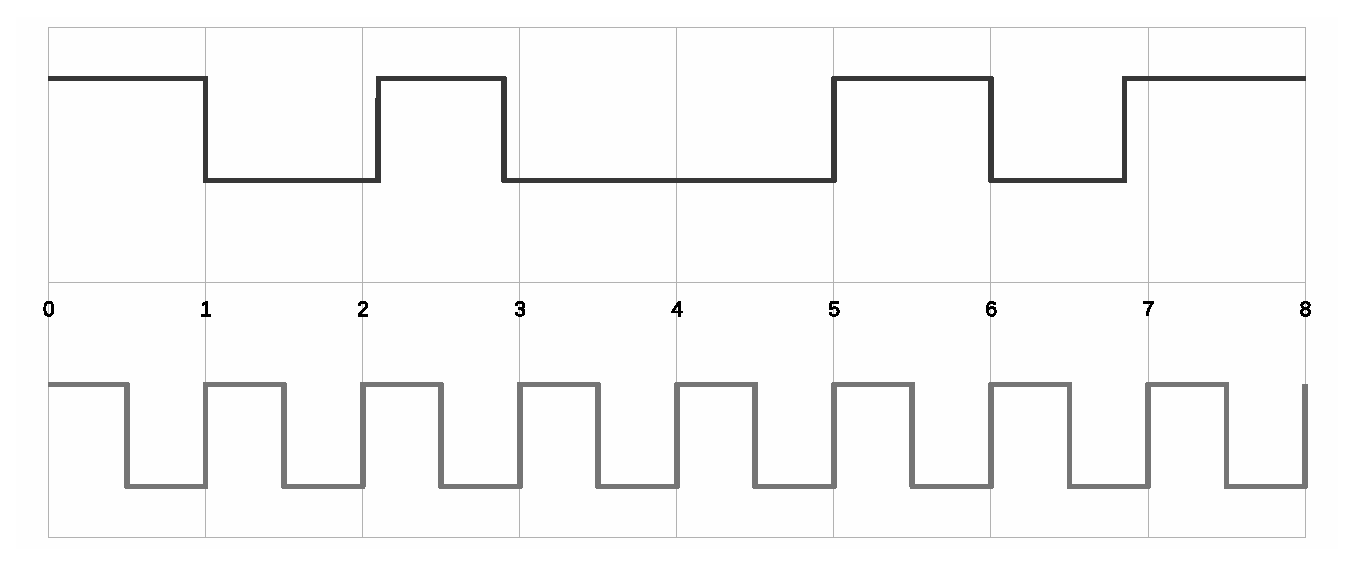
\includegraphics[width=0.9\linewidth,keepaspectratio]{fig/fig4_1.eps}
\caption{連続同期方式:伝送信号(上)と同期パルス(下)}\label{fig4_1}
\end{figure}

この方式を実現する単純な方法としては2本の伝送路を用意するということがあるが無駄が多い。このため、現在は1本の通信回線上にデータと同期パルスを重ねて送出する方法が広く用いられている。また、重ね合わせて送出するだけであり、元のデータにビット等を付加する必要がないため、長いデータを送出する際にも伝送効率がよい。

\subsection{非同期方式(調歩同期方式)}
非同期方式は\textbf{調歩同期方式}\index{ちょうほどうきほうしき@調歩同期方式}とも呼ばれる。これはデータの始まりを示すビットを付けてビット位置を知らせる手法である。

非同期方式の場合、通信が行われていないときには常に一定の電圧がかかっている。ここで、スタートビットと呼ばれるビットが電圧0として流れてくる。これがデータの始まりである。この後、予め定まった長さ毎に電圧を解釈し0または1のビットに割り当てていく。この部分をデータビットと呼ぶ。データビットを一定数(通常7bitか8bit)読んだら、次の同期のために電圧を1に戻す。この1に戻すビットのことをストップビットと呼ぶ。このように、予め長さを決めた上でデータの始端・終端で同期を取るのが非同期方式である。非同期方式とは同期式と異なる(同期式ではない)という意味であり、「同期処理自体が行われない」という意味ではない点に注意されたい。

図\ref{fig4_2}に、8bitの調歩同期方式の例を示す。これは図\ref{fig4_1}と同様、10100101というビット列を送った例である。平常時は1に相当する電圧がかかっている(-1から0)。次いでスタートビット(0から1)が来て、8bitのデータビット(1から9)が届く。ここで、2から3のように途中で値が変わっている場合、長い側の値を採用するのは連続同期方式と同様である。その後、ストップビットが届き(9から10)、平常の1の状態に戻る(10から11)。次のデータが開始したらまたスタートビットが届く(11から12)。なお、連続したデータを送る場合、平常に戻る箇所(10から11)はないこともある。
\begin{figure}[h]
\centering
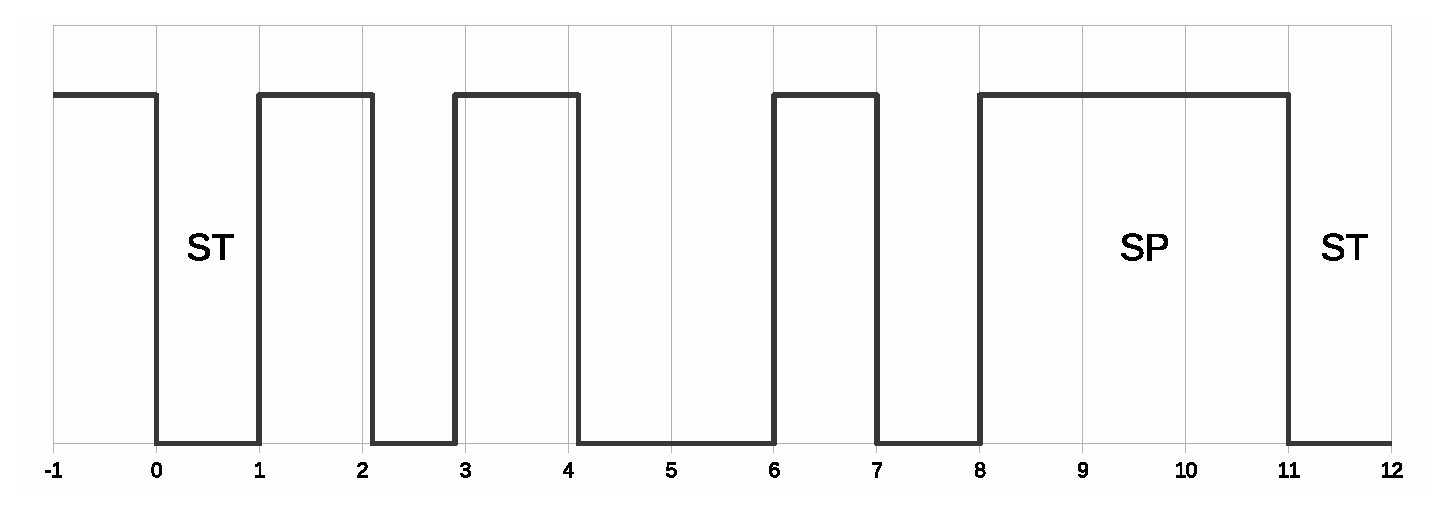
\includegraphics[width=0.9\linewidth,keepaspectratio]{fig/fig4_2.eps}
\caption{8bitの調歩同期方式:STはスタートビット・SPはストップビット}\label{fig4_2}
\end{figure}

調歩同期方式では一定のデータビット毎にスタートビットとストップビットが付加されるため通信の効率が落ちてしまう。一方で、同期パルス形式に比べより自由なタイミングで、場合によっては安価に環境を用意できるのが利点である。

\section{ブロック同期}
ビット同期によって各ビットが正しく識別できたとしても、データの開始や終了、区切りがわからなければ正しく解釈できない。そこで、データの区切り位置を送受信双方で合わせるのがブロック同期である。先の調歩同期方式ではビット列の解釈を合わせるとともにスタートビット・ストップビットによってデータの始点・終点を定められたため、調歩同期方式はブロック同期も行えるが、連続同期方式ではそうは行かない。

ブロック同期方式として\textbf{キャラクタ同期方式}\index{きゃらくたどうきほうしき@キャラクタ同期方式}と\textbf{フラグ同期方式}\index{ふらぐどうきほうしき@フラグ同期方式}(\textbf{フレーム同期方式}\index{ふれーむどうきほうしき@フレーム同期方式|see{フラグ同期方式}})を紹介する。

\subsection{キャラクタ同期方式}

キャラクタ同期方式は、その名前の示すとおり、文字の情報を送るときに多く使われる手法である。このため、キャラクタ同期方式は1オクテット毎にデータを送付する。この方式では、SYN(シン)キャラクタと呼ばれる制御コードを送ることでデータの先頭位置を示す。ここで、一般にSYNキャラクタは00010110で表される文字である(通例、通信時には低位のビットから送るため、受信順序は逆となる)。同期の確実性のためSYNキャラクタは2度以上続けて送られるのが普通である。

送信側ではデータを送信していないとき、常にSYNキャラクタを送り続ける。一方受信側では、このSYNキャラクタを監視することによって同期をとる。つまり、bit単位で見ていた調歩同期方式をoctet単位に変えたような動作である。順に送られ続けるビットからSYNキャラクタを見出し、ここをデータの区切りとすることで同期が確立する。一旦同期が確立すると、octet単位でデータを読み込み続け、SYNキャラクタ以外のパターンを受け取ったときにこれをデータとして解釈していく。

尚、キャラクタ同期方式は必ずしも文字だけに使われるわけではない。文字以外のデータもoctet単位に区切って送信することができる。このとき、SYNキャラクタと同じパターンが混在してしまうことがあるが、これはエスケープ処理としてDLE(デル)キャラクタを前に付加して送信する。受信側ではSYNキャラクタの前にDLEキャラクタを受信した場合、DLEキャラクタを破棄し、SYNキャラクタとして解釈するのである。

キャラクタ同期方式の場合、調歩同期方式と違って文字ごとにbitを付加する必要がなく、連続してデータを送信できるのが利点である(これはフレーム同期方式にも言えることだが)。

\subsection{フラグ同期方式(フレーム同期方式)}
フラグ同期方式は、あらかじめ決められた同期用のビットパターン(フラグパターンと呼ばれ、01111110が使われる)を送信データの始めと終わりに付けて送り出す方式である。受信側では、このデータを監視し、フラグを検出すると次のフラグまでの間を一連のデータとして解釈する。キャラクタ同期との違いは、データの区切りを8ビットと定めていないため8ビットの倍数とは限らない長さのデータを送ることができるという点である。この点を除けば、SYNがフラグパターンに変わったキャラクタ同期方式と考えても(多少の差異はあれど)間違いではない。

キャラクタ同期方式との差異として挙げられるのはエスケープの方式である。フラグ同期方式ではフラグパターンに1が6連続しているという点に着目し、送信時に1が5ビット連続したら強制的に0を挿入する。逆に、受信側では1が5ビット連続した後の0を取り除く。この決まりによりデータを間違いなく受信することができる。

フラグ同期方式はキャラクタ同期方式に比べエスケープのビット数が少ないことや可変長で送信できることなどから、伝送効率が良い手法である。

\section*{演習問題}
\begin{problems}
\item 図\ref{fig4_3}はbit同期の単位時間を1とした場合の入力電圧を示したものである。入力電圧1(=0.5以上)がbitの1に、0(=0.5未満)がbitの0に対応するとき、この図から抽出されるべき8ビットのビット列を答えよ。尚、入力電圧データにはノイズがある点に注意せよ。
\begin{figure}[h]
\centering
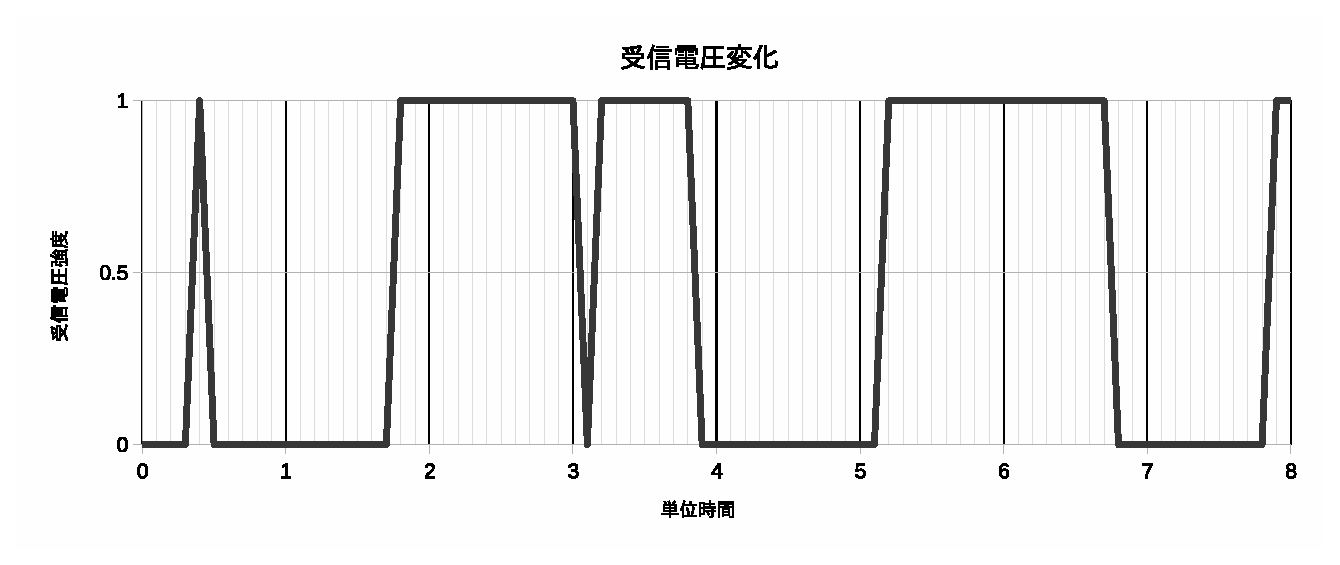
\includegraphics[width=0.9\linewidth,keepaspectratio]{fig/fig4_3.eps}
\caption{入力電圧データ}\label{fig4_3}
\end{figure}

\item 7bit単位でデータが区切られる調歩同期方式で70kBのデータを送信したい。このとき、調歩同期方式で付加されるビットを含めた実通信量は何バイトになるか。

\item ある通信においてブロック同期が適切に行われなかった結果、最初の4bitが読まれず、データ列が16進表記で"1A 2B 4D F0"となった。最初の読まれなかった4bitが16進表記でCであり、最後の0が不要なデータであった場合、この正しいデータ列はどのようになるか。
\end{problems}
